\chapter{Software}
\label{chp:S}

%%%%%%%%%%%%%%%%%%%%%%%%%%%%%%%%%%%%%%%%%%%%%%%%%%%%%%%%%%%%%%%%%%%%%%%
\section{Motivation}

\subsection{Software}

MSC.Marc Mentat 2019 is used to construct and define the templates, units and bodies. MSC.Marc Mentat 2019 is used to model the materials and their behaviour. Marc is capable of advanced non-linear analysis.

Python 3.6 is used to construct a modelling pipeline. Packages are available that allow for the integration of Python and Marc. Many advanced numerical analysis packages are also available for Python.

\subsection{Materials}

Mold Star 15 SLOW is selected as the material to be digitally modelled for the purposes of the project. Mold Star 15 has a hyper-elastic non-linear response. It is suitable for inflation while being capable of supporting itself at the relevant scale of construction.

\subsection{Assumptions}

A 2D modeling approach is followed. 2D modeling reduces complexity and computational requirements. 2D modeling is analogous to real-world behaviour under appropriate circumstances \cite{Ellis2020, Joubert2020}.

A complete unit boundary of varying thickness is always present. External elements and their neighbours for a specified range inwards are always excluded from being removed during unit generation. A complete unit boundary prevents any unwanted gaps when units are used to construct bodies. A complete unit boundary simplifies the process of applying boundary conditions.

Mesh refinement during a simulation is not possible with the current software architecture. The construction of the units also defines the element and node indices and coordinates. The indices and coordinates are referenced and used throughout the simulation and data retrieval. Mesh refinement would change the indices and coordinates, rendering the software incapable of interpreting the simulations. More accurate results may be achieved by running simulations at higher element resolutions. Higher element resolutions will result in different unit configurations.

Free-floating elements are eliminated during unit generation. Therefore fewer unique combinations exist than an $n Choose r$ calculation would arrive at. It is not possible to determine exactly how many unique possible combinations exist without generating all of them. This unnecessary and computationally expensive. The result of the $n Choose r$ calculation is used as an estimate of the number of possible unique combinations.

Material properties for Mold Star 15 are initially obtained from previous work \cite{Ellis2020}. Due to the COVID-19 pandemic, testing facilities were not available at an appropriate time to perform material testing before software implementation. Material testing is intended to occur before the completion of the project to verify the material properties used.

\section{Method}

Figure~\ref{fig:sp} roughly illustrates the current software pipeline. Elaborative figures are found in Appendix~\ref{chp:softpipe}.

\begin{figure}[H]
\begin{center}
	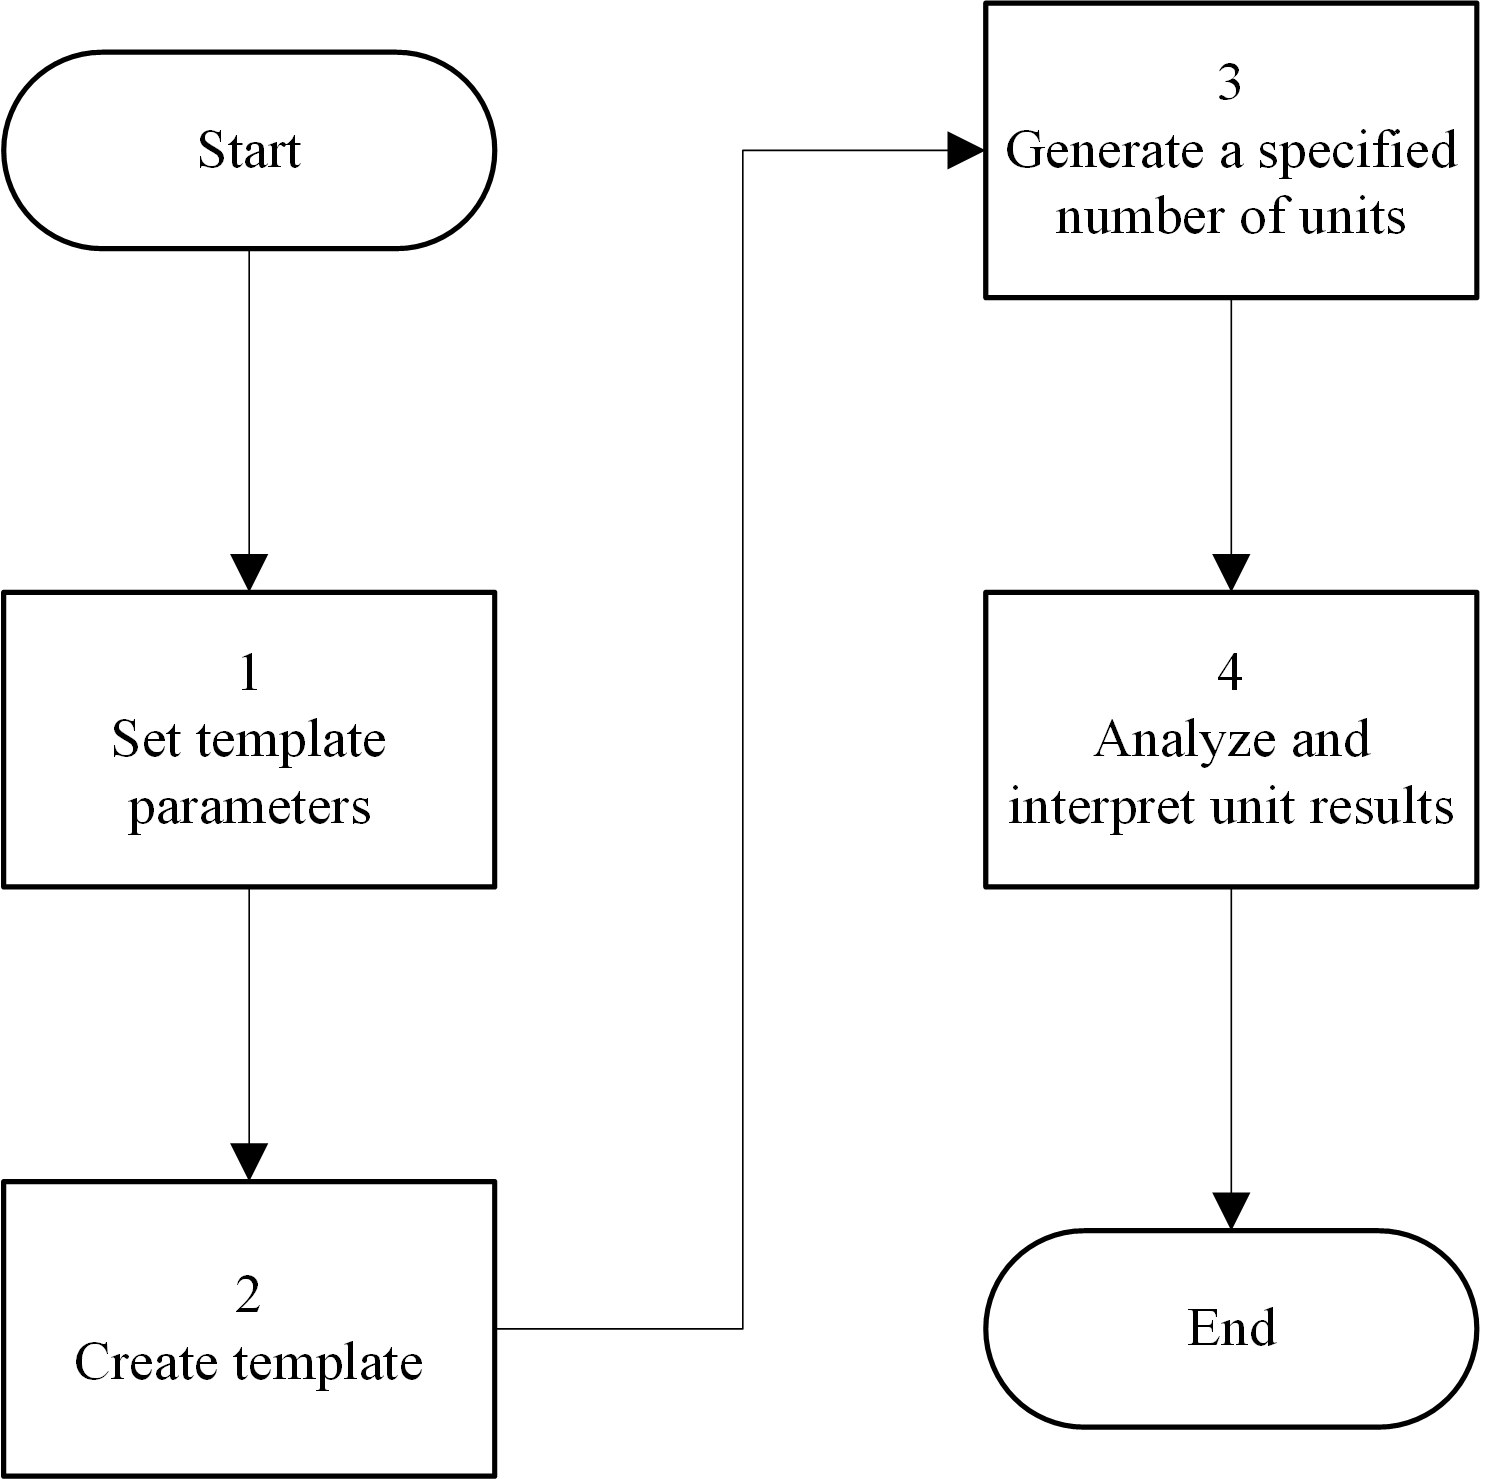
\includegraphics[width=0.7\textwidth]{sp.png}
	\caption{Software Pipeline}
	\label{fig:sp}
\end{center}
\end{figure}

\subsection{File Management}

File management is an important component of the software structure. A large number of files are generated during simulations. Each model file has a number of files associated with it. Many model files may be generated during a simulation. Every simulation with new parameters requires new addresses and forms of identification. Figure~\ref{fig:fh} illustrates the file hierarchy implemented in the software. Dotted lines indicate components that are still to be implemented. Table~\ref{tab:fhk} serves as a key for Figure~\ref{fig:fh}.

\begin{landscape}
	\begin{figure}
  		\centering
  		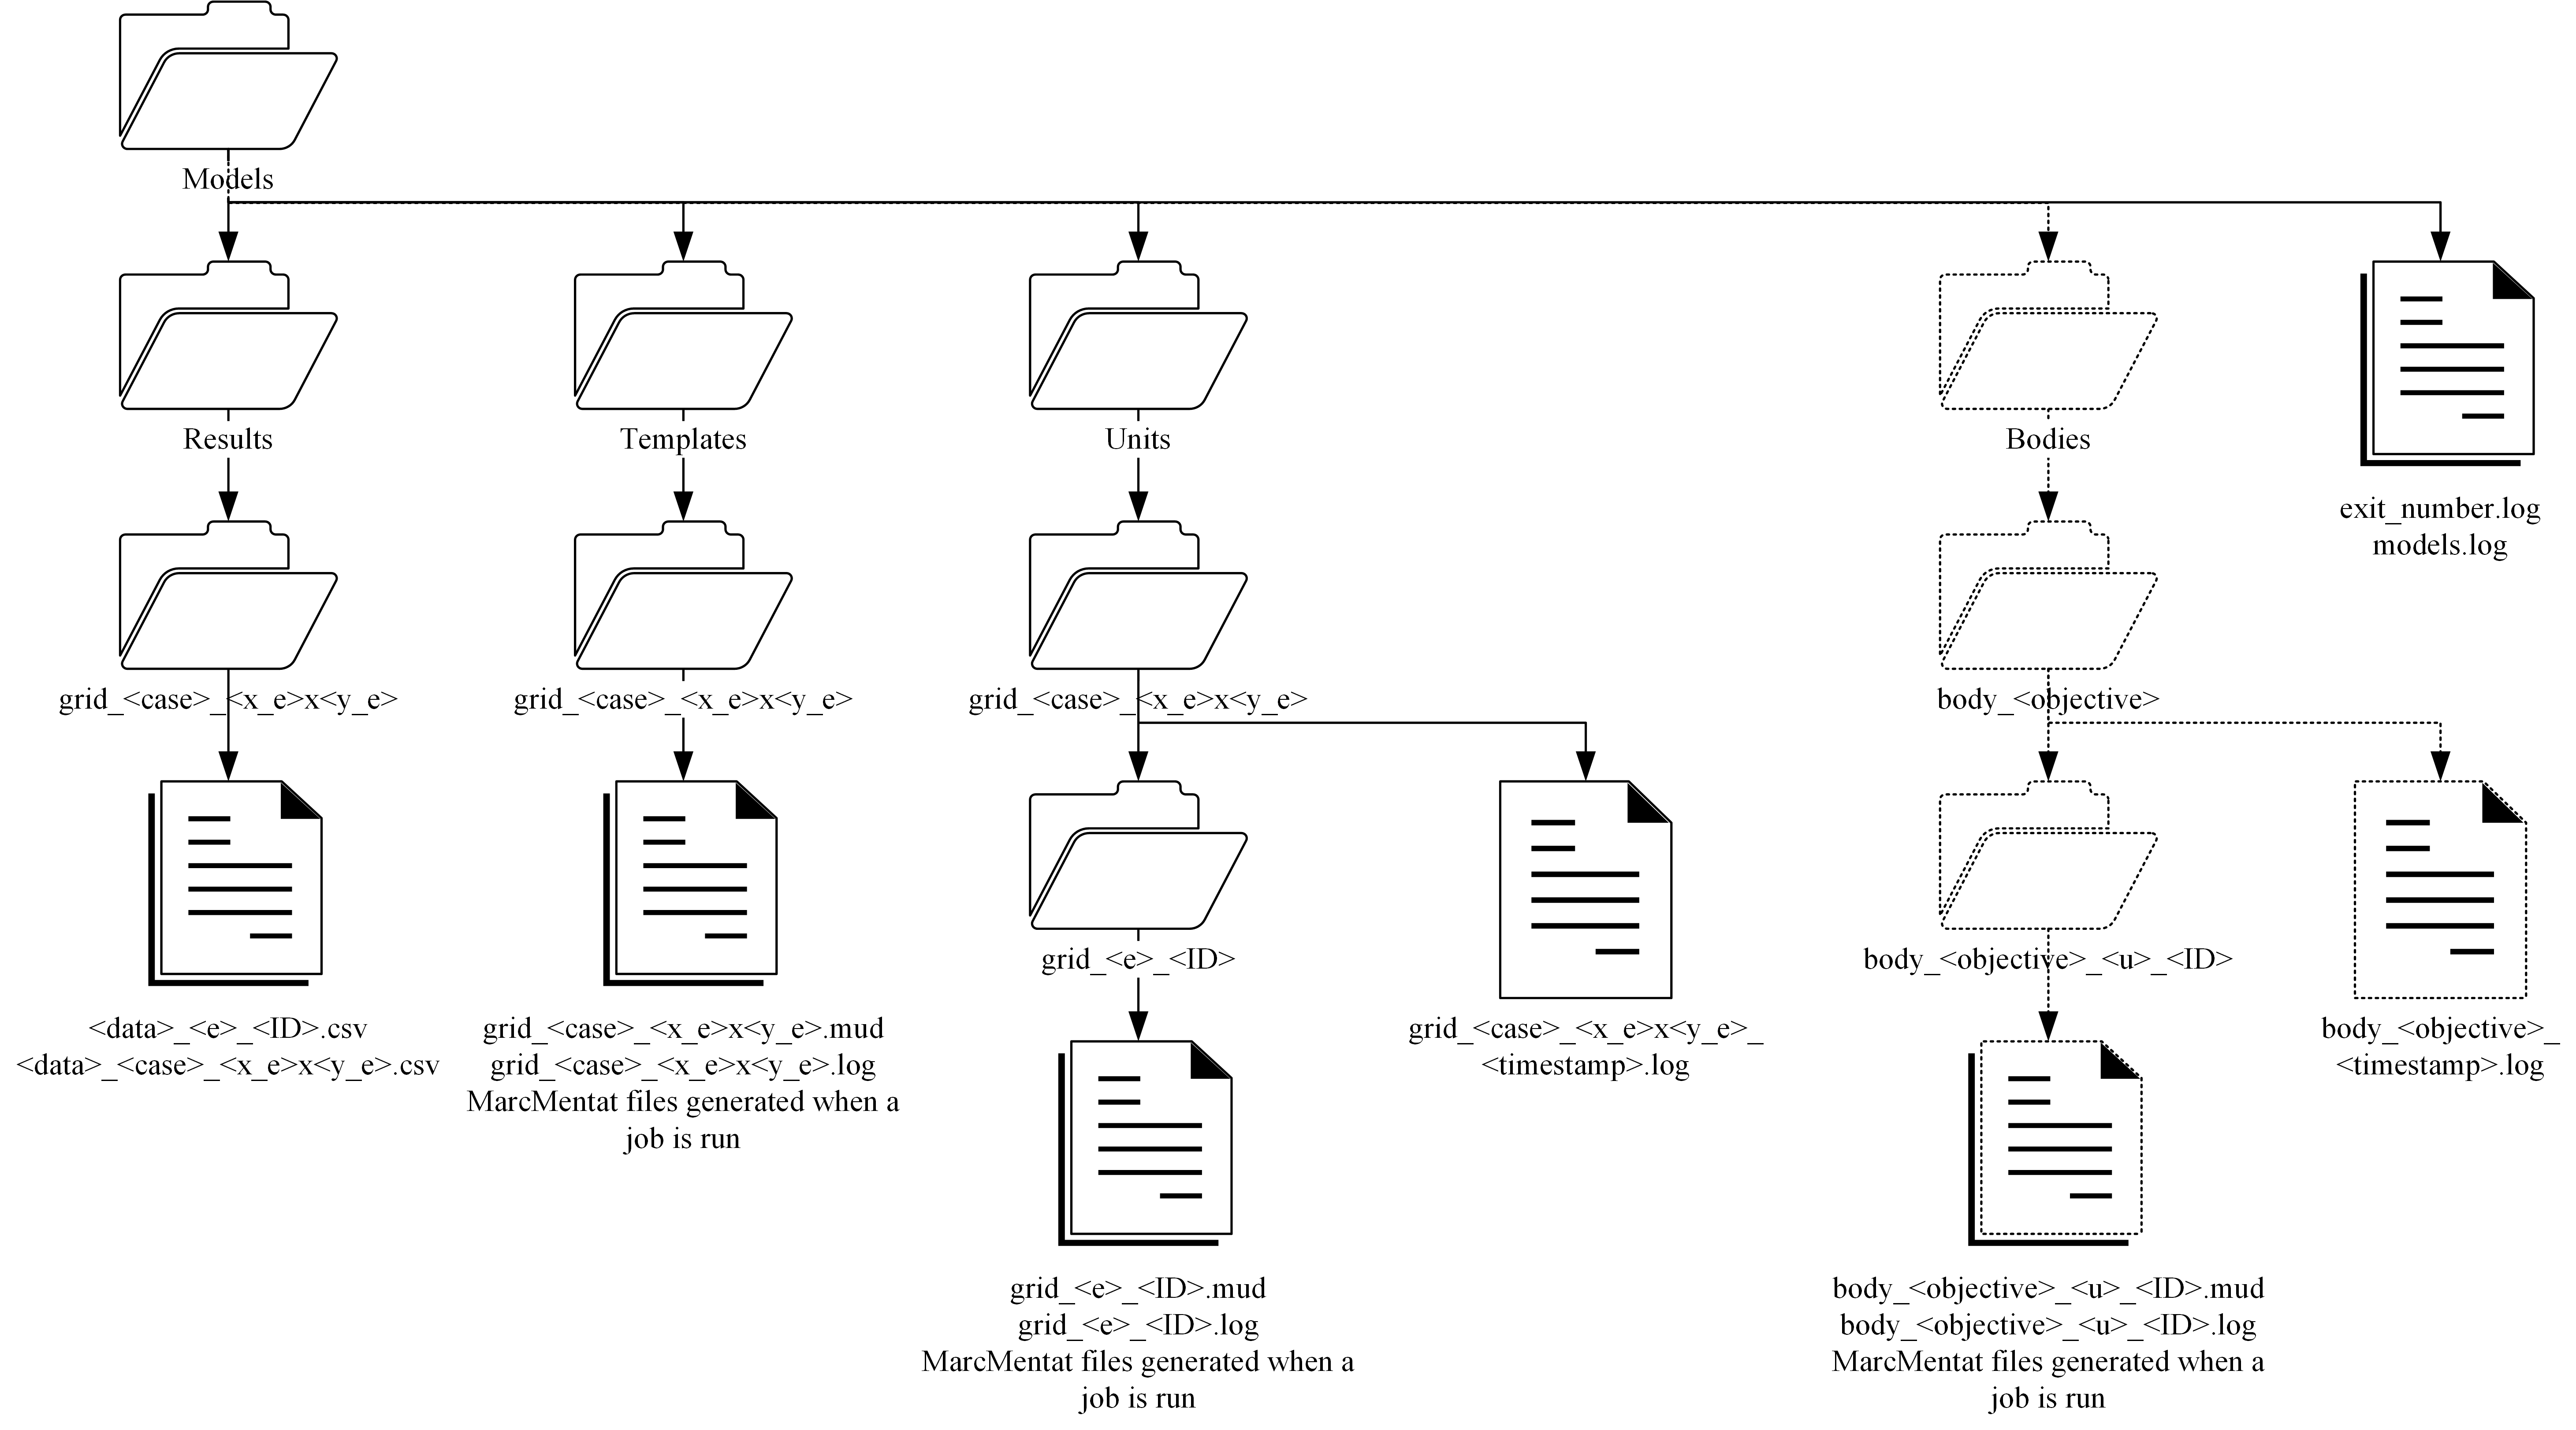
\includegraphics[width=1.6\textwidth]{file.png}
  		\caption{File Hierarchy}
  		\label{fig:fh}
	\end{figure}
\end{landscape}

\begin{table}[H]
\centering
\caption{File Hierarchy Key}
\label{tab:fhk}
\begin{tabular}{|l|l|c|}
\hline
\textbf{Name} &
  \textbf{Description} &
  \multicolumn{1}{l|}{\textbf{Example}} \\ \hline
case &
  The unit case identifier &
  1 \\ \hline
x\_e &
  \begin{tabular}[c]{@{}l@{}}The number of elements\\ in the x-direction\end{tabular} &
  5 \\ \hline
y\_e &
  \begin{tabular}[c]{@{}l@{}}The number of elements\\ in the y-direction\end{tabular} &
  5 \\ \hline
data &
  The type of data stored &
  Reaction Force \\ \hline
e &
  \begin{tabular}[c]{@{}l@{}}The number of elements\\ removed\end{tabular} &
  5 \\ \hline
ID &
  The unique unit ID &
  \begin{tabular}[c]{@{}c@{}}4121ab03c09f703b\\ eb534ab74aa3c079\end{tabular} \\ \hline
timestamp & \begin{tabular}[c]{@{}l@{}}The timestamp of the\\ start of the simulation\end{tabular} & \begin{tabular}[c]{@{}c@{}}2020-05-20\\ --15-20-55\end{tabular} \\ \hline
objective &
  \begin{tabular}[c]{@{}l@{}}The body objective\\ identifier\end{tabular} &
  A \\ \hline
u &
  \begin{tabular}[c]{@{}l@{}}The number of units\\ used to construct the\\ body\end{tabular} &
  10 \\ \hline
\end{tabular}
\end{table}

The software code is structured as a Python library. Python libraries allow for intuitive organisation and hierarchical construction of code. Relevant functions are grouped together. Sub-grouping is possible where required. Figure~\ref{fig:pl} illustrates the Python library structure implemented for this project's code. Table~\ref{tab:pld} describes the relevant function libraries.

\begin{figure}[H]
\begin{center}
	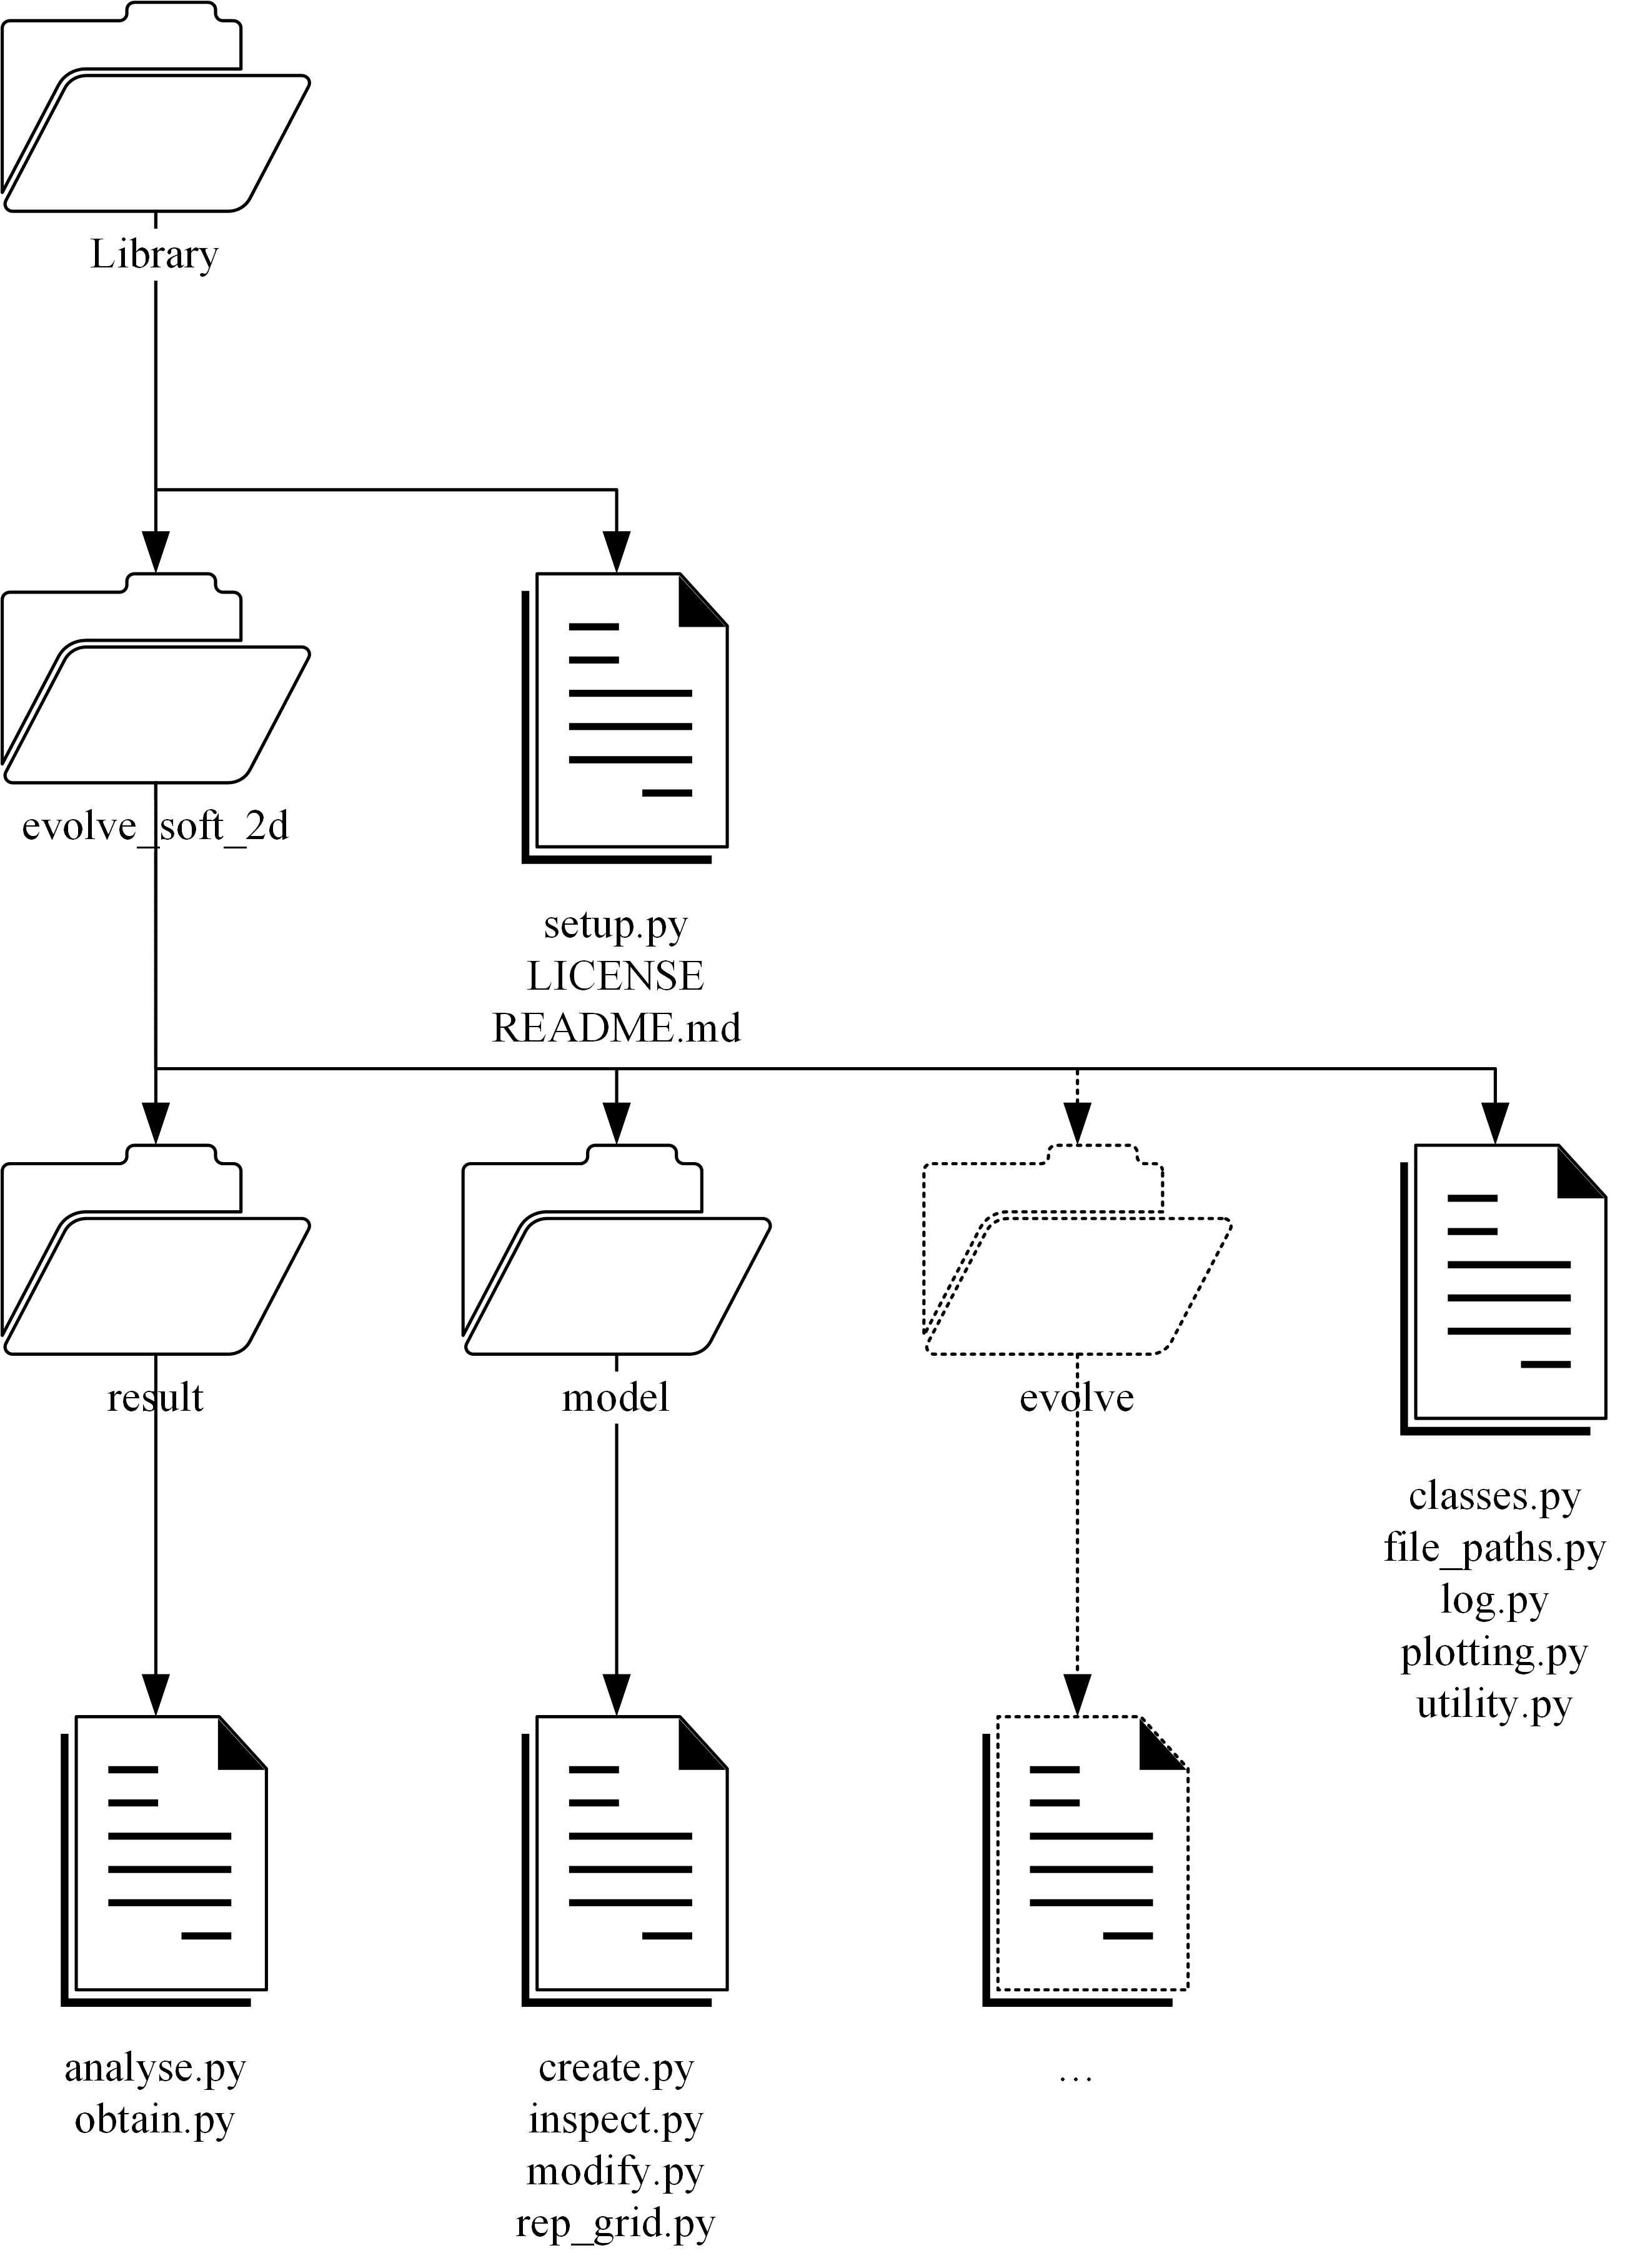
\includegraphics[width=1\textwidth]{pythonlib.png}
	\caption{Python Library}
	\label{fig:pl}
\end{center}
\end{figure}

% Please add the following required packages to your document preamble:
% \usepackage{booktabs}
\begin{table}[]
\centering
\caption{Python Library Description}
\label{tab:pld}
\begin{tabular}{@{}ll@{}}
\toprule
\textbf{Name}    & \textbf{Description}                                       \\ \midrule
evolve\_soft\_2d & The main library folder                                    \\
result       & \begin{tabular}[c]{@{}l@{}}The folder containing functions related to obtaining and\\ analysing results\end{tabular} \\
model        & \begin{tabular}[c]{@{}l@{}}The folder containing functions related to creating and\\ modifying models\end{tabular}   \\
evolve           & The folder containing functions related to evolving models \\
classes.py   & \begin{tabular}[c]{@{}l@{}}The object classes, their related functions, and example\\ material models\end{tabular}   \\
file\_paths.py   & The file path generative functions and base file paths     \\
log.py           & The logging formatting and functions                       \\
plotting.py      & The plotting functions                                     \\
utility.py       & Utility functions for multiple purposes                    \\
analyse.py       & Result analysis functions                                  \\
obtain.py        & Result obtainment functions                                \\
create.py        & Simulation and template creation functions                 \\
inspect.py       & Model inspection functions                                 \\
modify.py        & Model creation and modification functions                  \\
rep\_grid.py & \begin{tabular}[c]{@{}l@{}}The representative grid creation and modification\\ functions\end{tabular}                \\ \bottomrule
\end{tabular}
\end{table}

\subsection{Material Properties}

An Ogden material model of Mold Star 15 is used. Material model parameters are obtained from \cite{Ellis2020}. Material model parameters are shown in Table~\ref{tab:ms15om} and applied to Equation~\ref{eq:om}.

% Please add the following required packages to your document preamble:
% \usepackage{booktabs}
\begin{table}[H]
\centering
\caption{Mold Star 15 Ogden Parameters \cite{Ellis2020}}
\label{tab:ms15om}
\begin{tabular}{@{}lrrr@{}}
\toprule
\textbf{Parameter} & \multicolumn{1}{c}{\textbf{1}} & \multicolumn{1}{c}{\textbf{2}} & \multicolumn{1}{c}{\textbf{3}} \\ \midrule
$\mu$              & -6.50266e-06                   & 0.216863                       & 0.00137158                     \\
$\alpha$           & -21.322                        & 1.1797                         & 4.88396                        \\ \bottomrule
\end{tabular}
\end{table}

\subsection{Units}

Certain template parameters are required to be provided by the user. Other template parameters are calculated and/or generated when the template class object is defined. Relevant template parameters and example parameters are outlined in Table~\ref{tab:tcop}.

% Please add the following required packages to your document preamble:
% \usepackage{graphicx}
\begin{table}[H]
\caption{Template Class Object Parameters}
\label{tab:tcop}
\resizebox{\textwidth}{!}{%
\begin{tabular}{|l|l|l|l|c|}
\hline
\textbf{Parameter} &
  \textbf{Data Type} &
  \textbf{Description} &
  \textbf{Source} &
  \multicolumn{1}{l|}{\textbf{Example}} \\ \hline
case &
  int &
  The unit case identifier &
  User-defined &
  1 \\ \hline
x0 &
  int &
  The initial x-coordinate &
  User-defined &
  0 \\ \hline
y0 &
  int &
  The initial y-coordinate &
  User-defined &
  0 \\ \hline
x\_n &
  int &
  \begin{tabular}[c]{@{}l@{}}The number of nodes in\\ the x-direction\end{tabular} &
  User-defined &
  6 \\ \hline
y\_n &
  int &
  \begin{tabular}[c]{@{}l@{}}The number of nodes in\\ the y-direction\end{tabular} &
  User-defined &
  6 \\ \hline
ogd\_mat &
  ogd\_mat &
  \begin{tabular}[c]{@{}l@{}}The Ogden material\\ model\end{tabular} &
  User-defined &
  mold\_star\_15 \\ \hline
n\_steps &
  int &
  \begin{tabular}[c]{@{}l@{}}The number of steps in\\ the second of the\\ simulation\end{tabular} &
  User-defined &
  4 \\ \hline
tab\_nam &
  str &
  \begin{tabular}[c]{@{}l@{}}The name of the table\\ containing the function\\ of the load to be applied\end{tabular} &
  User-defined &
  ramp\_input \\ \hline
apply &
  float &
  \begin{tabular}[c]{@{}l@{}}The conditions to be\\ applied to the unit\\ template\end{tabular} &
  User-defined &
  $\frac{y_{n}-1}{2}$ \\ \hline
run\_success &
  bool &
  \begin{tabular}[c]{@{}l@{}}The success of the\\ unit template's run\end{tabular} &
  Obtained &
  True \\ \hline
c\_e &
  float &
  \begin{tabular}[c]{@{}l@{}}The constraint energy\\ of the unit template\end{tabular} &
  Obtained &
  6462952.804663594 \\ \hline
i\_e &
  float &
  \begin{tabular}[c]{@{}l@{}}The internal energy\\ of the unit template\end{tabular} &
  Obtained &
  1505641.7999267578 \\ \hline
n\_n &
  int &
  \begin{tabular}[c]{@{}l@{}}The total number of\\ nodes\end{tabular} &
  $x_{n}\times y_{n}$ &
  36 \\ \hline
x\_e &
  int &
  \begin{tabular}[c]{@{}l@{}}The number of\\ elements in the\\ x-direction\end{tabular} &
  $x_{n}-1$ &
  5 \\ \hline
y\_e &
  int &
  \begin{tabular}[c]{@{}l@{}}The number of\\ elements in the\\ y-direction\end{tabular} &
  $y_{n}-1$ &
  5 \\ \hline
n\_e &
  int &
  \begin{tabular}[c]{@{}l@{}}The total number of\\ elements\end{tabular} &
  $x_{e}\times y_{e}$ &
  25 \\ \hline
n\_e\_l &
  str &
  \begin{tabular}[c]{@{}l@{}}The total number of\\ elements as a string\\ label\end{tabular} &
  Obtained &
  5x5 \\ \hline
e\_internal &
  list &
  \begin{tabular}[c]{@{}l@{}}The list of internal\\ elements\end{tabular} &
  Obtained &
  \begin{tabular}[c]{@{}c@{}}{[}7, 8, 9,\\ 12, 13, 14,\\ 17, 18, 19{]}\end{tabular} \\ \hline
n\_external &
  list &
  \begin{tabular}[c]{@{}l@{}}The list of external\\ nodes\end{tabular} &
  Obtained &
  \begin{tabular}[c]{@{}c@{}}{[}1, 2, 3, 4, 5, 6,\\ 7, 12, 13, 18,\\ 19, 24, 25, 30,\\ 31, 32, 33, 34, 35, 36{]}\end{tabular} \\ \hline
grid &
  list &
  \begin{tabular}[c]{@{}l@{}}The representative\\ grid of ones\end{tabular} &
  Obtained &
  \begin{tabular}[c]{@{}c@{}}{[}{[}1, 1, 1, 1, 1{]},\\ {[}1, 1, 1, 1, 1{]},\\ {[}1, 1, 1, 1, 1{]},\\ {[}1, 1, 1, 1, 1{]},\\ {[}1, 1, 1, 1, 1{]}{]}\end{tabular} \\ \hline
fp\_t\_... &
  str &
  \begin{tabular}[c]{@{}l@{}}The various file paths\\ associated with the\\ template\end{tabular} &
  Obtained &
  \begin{tabular}[c]{@{}c@{}}C:...\textbackslash{}Templates\\ \textbackslash{}grid\_1\_5x5\\ \textbackslash{}grid\_1\_5x5.mud\end{tabular} \\ \hline
\end{tabular}%
}
\end{table}

A unit template is generated in Marc Mentat according to the template parameters. Units are 2D meshes constructed from square elements. A template is a solid grid with all boundary conditions and other properties defined. Figure~\ref{fig:ut1} illustrates an example template.

\begin{figure}[H]
	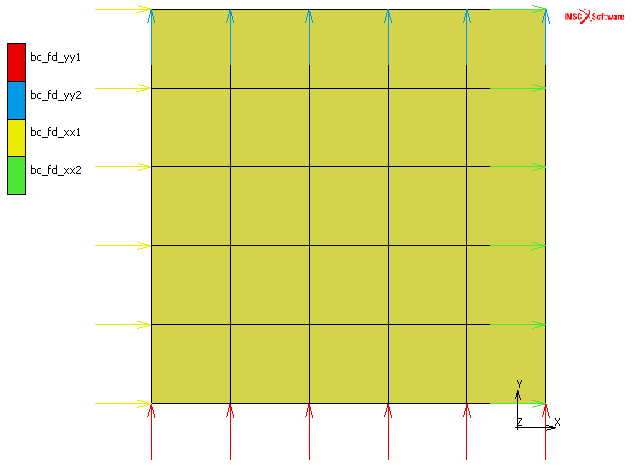
\includegraphics[width=1\textwidth]{grid_1_5x5.png}
	\caption{Unit Template For Case 1}
	\label{fig:ut1}
\end{figure}

A specified number of unique units are generated, run and analysed. A check is performed to determine that no more unique units are requested than theoretically possible. Units are defined by removing random internal elements. Free-floating elements are identified and removed. Free-floating elements are defined as any elements that do not share at least two node connections with a single other node. Figure~\ref{fig:ffee} illustrates some examples.

\begin{figure}[H]
  \centering
  \medskip
  \begin{subfigure}[t]{.3\linewidth}
    \centering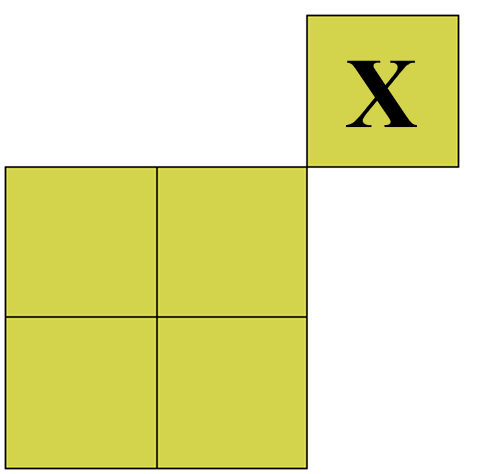
\includegraphics[width=.8\linewidth]{free1.png}
    \caption{Element X is recognised as free-floating and will be removed.}
  \end{subfigure}
  \begin{subfigure}[t]{.3\linewidth}
    \centering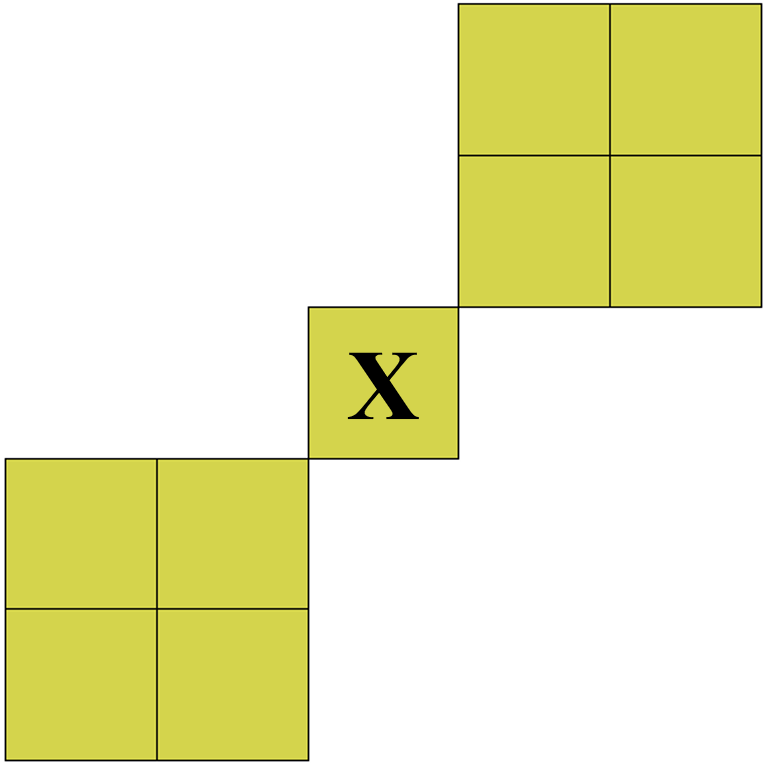
\includegraphics[width=.8\linewidth]{free2.png}
    \caption{Element X is recognised as free-floating and will be removed.}
  \end{subfigure}
  \begin{subfigure}[t]{.3\linewidth}
    \centering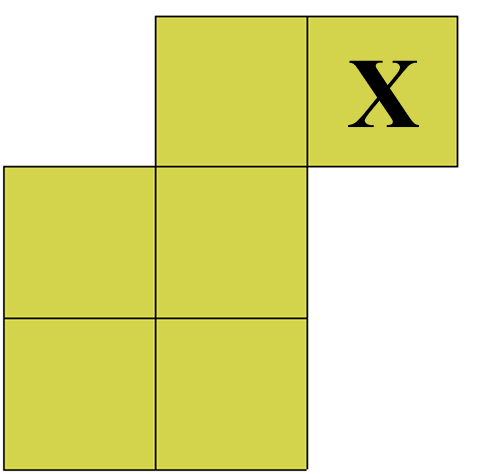
\includegraphics[width=.8\linewidth]{notfree1.png}
    \caption{Element X is not recognised as free-floating and will remain.}
  \end{subfigure}
  \caption{Free-Floating Element Examples}
  \label{fig:ffee}
\end{figure}

The number of elements removed and the element IDs of the removed elements are used to generate a unique ID for each unit. Unit parameters are saved. Relevant unit parameters and example parameters are outlined in Table~\ref{tab:ucop}. Units are run and evaluated. Displacement, reaction force and strain energy density data are extracted from each unit and used to evaluate them.

% Please add the following required packages to your document preamble:
% \usepackage{graphicx}
\begin{table}[H]
\caption{Unit Class Object Parameters}
\label{tab:ucop}
\resizebox{\textwidth}{!}{%
\begin{tabular}{|l|l|l|l|c|}
\hline
\textbf{Parameter} &
  \textbf{Data Type} &
  \textbf{Description} &
  \textbf{Source} &
  \multicolumn{1}{l|}{\textbf{Example}} \\ \hline
template &
  template &
  \begin{tabular}[c]{@{}l@{}}The unit template\\ parameters\end{tabular} &
  User-defined &
  temp\_1 \\ \hline
rem &
  list &
  \begin{tabular}[c]{@{}l@{}}The list of elements\\ removed from the\\ unit\end{tabular} &
  Obtained &
  {[}7, 8, 13, 18, 19{]} \\ \hline
grid &
  list &
  \begin{tabular}[c]{@{}l@{}}The representative\\ grid with the\\ elements removed\end{tabular} &
  Obtained &
  \begin{tabular}[c]{@{}c@{}}{[}{[}1, 1, 1, 1, 1{]},\\ {[}1, 1, 0, 0, 1{]},\\ {[}1, 1, 0, 1, 1{]},\\ {[}1, 0, 0, 1, 1{]},\\ {[}1, 1, 1, 1, 1{]}{]}\end{tabular} \\ \hline
run\_success &
  bool &
  \begin{tabular}[c]{@{}l@{}}The success of the\\ unit's run\end{tabular} &
  Obtained &
  True \\ \hline
c\_e &
  float &
  \begin{tabular}[c]{@{}l@{}}The constraint\\ energy of the unit\end{tabular} &
  Obtained &
  2951.728374235662 \\ \hline
i\_e &
  float &
  \begin{tabular}[c]{@{}l@{}}The internal\\ energy of the unit\end{tabular} &
  Obtained &
  1530.943825491704 \\ \hline
u\_id &
  str &
  The unique unit ID &
  Obtained &
  \begin{tabular}[c]{@{}c@{}}5\_4121ab03c09f703\\ beb534ab74aa3c079\end{tabular} \\ \hline
fp\_u\_... &
  str &
  \begin{tabular}[c]{@{}l@{}}The various file\\ paths associated\\ with the template\end{tabular} &
  Obtained &
  \begin{tabular}[c]{@{}c@{}}C:..\textbackslash{}Units\textbackslash{}grid\_1\_5x5\\ \textbackslash{}grid\_5\_4121ab03c09f703\\ beb534ab74aa3c079\\ \textbackslash{}grid\_5\_4121ab03c09f703\\ beb534ab74aa3c079.mud\end{tabular} \\ \hline
\end{tabular}%
}
\end{table}

Displacement and reaction force nodal values are used to calculate constraint energy. Constraint energy is defined as

\begin{equation}
	\label{eq:ce}
	E=\sum_{i=1}^{n}F_{i}d_{i}
\end{equation}

where

\begin{itemize}
	\item $i$ is any node on the external boundary
	\item $n$ is the total number of nodes
	\item $F$ is the reaction force at the node
	\item $d$ is the displacement at the node
\end{itemize}

Different results are desired for different cases. Specific cases are discussed in Section~\ref{sec:cas}.

\section{Cases}
\label{sec:cas}

Generic properties are applied to each template. Generic properties include a ramp table representative of a simple $y=x$ equation used to apply displacements over time. Plane strain geometric properties are added. Solid state contact body properties are added. A static loadcase is added. A structural job is added requesting total strain energy density outputs.

\subsection{Case 1}

Case 1 is reflective of pure stress in a single direction. The y-direction is arbitrarily chosen. If extension in the x-direction is required, a unit may be rotated by 90\textdegree . Case 1 is obtained from \cite{Cook2002}. Case 1 is selected because of the usefulness of simple linear extension and the lack of rigid body modes. Boundary conditions are defined in Table~\ref{tab:c1bc} and illustrated in Figure~\ref{fig:c1}.

\begin{table}[H]
\centering
\caption{Case 1 Boundary Conditions \cite{Cook2002}}
\label{tab:c1bc}
\begin{tabular}{lccc}
\hline
\multicolumn{1}{c}{\textbf{AB}} & \textbf{BC}               & \textbf{CD}               & \textbf{DA}               \\ \hline
$u=0$                           & \multicolumn{1}{r}{$v=a$} & \multicolumn{1}{r}{$u=0$} & \multicolumn{1}{r}{$v=0$} \\ \hline
\end{tabular}
\end{table}

\begin{figure}[H]
	\centering
	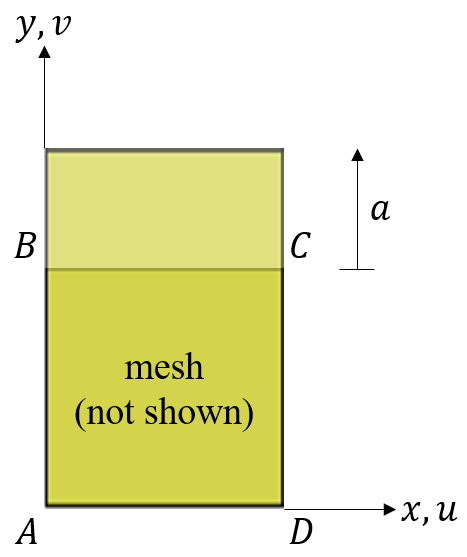
\includegraphics[width=0.5\textwidth]{case1.png}
	\caption{Case 1}
	\label{fig:c1}
\end{figure}

Successful units have comparatively low energy in the y-direction and near zero energy in the x-direction. Comparatively low energy in the y-direction for a constant displacement boundary condition implies a lower reaction force. A comparatively lower reaction force implies a smaller force required to obtain the desired displacement. Near zero energy in the x-direction for a fixed zero displacement boundary condition implies a low reaction force. A low reaction force implies a low resistance to being constrained in the x-direction.

Figure~\ref{fig:cesp} shows the distribution of 100 units' constraint energy in the x- and y-directions. Elements in the lower left area of the graph may be suitable candidates for case 1.

\begin{figure}[H]
	\centering
	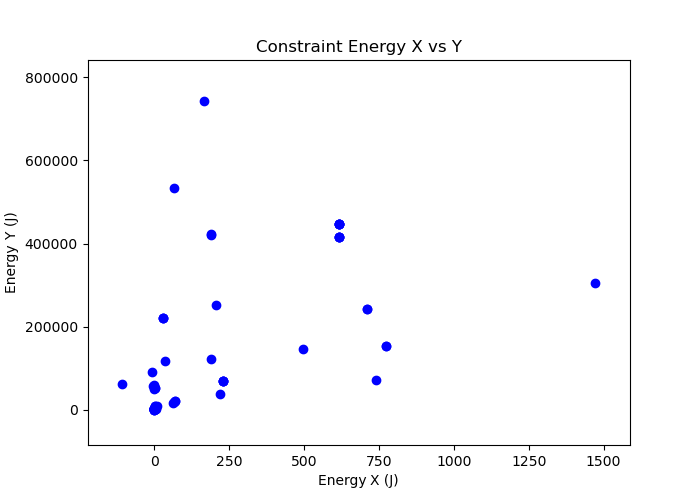
\includegraphics[width=1\textwidth]{c_e_x_vs_y.png}
	\caption{Constraint Energy Scatter Plot}
	\label{fig:cesp}
\end{figure}

\subsection{Case 2}

Case 2 is reflective of pure shear strain. Case 2 is obtained from \cite{Cook2002}. Case 1 is selected because of the usefulness of shear distortion and the lack of rigid body modes. Boundary conditions are defined in Table~\ref{tab:c2bc} and illustrated in Figure~\ref{fig:c2}.

\begin{table}[H]
\centering
\caption{Case 2 Boundary Conditions \cite{Cook2002}}
\label{tab:c2bc}
\begin{tabular}{lccc}
\hline
\multicolumn{1}{c}{\textbf{AB}} & \textbf{BC}               & \textbf{CD}               & \textbf{DA}               \\ \hline
$v=0$                           & \multicolumn{1}{r}{$u=a$} & \multicolumn{1}{r}{$v=0$} & \multicolumn{1}{r}{$u=0$} \\ \hline
\end{tabular}
\end{table}

\begin{figure}[H]
	\centering
	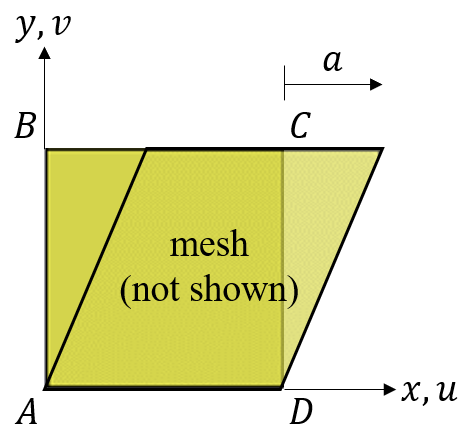
\includegraphics[width=0.5\textwidth]{case2.png}
	\caption{Case 2}
	\label{fig:c2}
\end{figure}